\documentclass{report}

\usepackage{apalike}
\usepackage{graphicx}

\title{replace title}
\author{replace author}
\date{replace date}

\begin{document}
\maketitle
\tableofcontents
\listoffigures

\chapter{Introduction}

\chapter{Executive Summary}
\section{Planning}
\subsection{Approach}
\subsection{Scope}
\subsection{Objectives}
\section{Methodology}
\subsection{Information Gathering}
\subsection{System Attacks}
\section{Summary of Findings}

\chapter{Key Findings}
\section{Auction Site}
This section covers the vulnerabilities found with the user-facing auction site.
\subsection{Path Traversal}
\subsubsection{Security Implications / Risk Level}
Path traversal allows for arbitrary file read across the system, for any files readable by the apache user (www-data). This is dangerous as it could potentially leak sensitive company data, as well as user data. If combined with other vulnerabilities, such as incorrect permissions on log files, it is possible to achieve Remote Code Execution through malicious log read/write.\\
Overall, the execution of this exploit is trivial, and the repercussions are potentially serious but not disasterous. Due to this, the risk level of this exploit is evaluated to be \textbf{medium}.
\subsubsection{Cause of Vulnerability}
The vulnerability is caused by the method used to retrieve and display image files on the website. Instead of directly referencing the image file through the 'src' field on an 'img' HTML tag, a PHP script is instead used to include the file.\\ 
While using PHP include scripts may not normally be dangerous, the file name to be retrieved can be edited by the user, allowing them to easily select which file should be displayed. A lack of filter/extension whitelist makes this even more potent.
\subsubsection{Steps to Replicate}
\begin{itemize}
		\item Firstly the inspect element tool in Mozilla Firefox was used to inspect an image, revealing the image URL (Fig. 3.1).
		\item The image URL could then be opened, showing the ASCII representation of the binary content for the image file (Fig. 3.2).
		\item Finally, the URL parameter 'file' could be replaced with a file path, allowing for arbitrary file read. In this example, the ../ operator was used to go up directories until root, and then the /etc/passwd file was navigated to (Fig. 3.3).
\end{itemize}
\begin{figure}
	\centering
	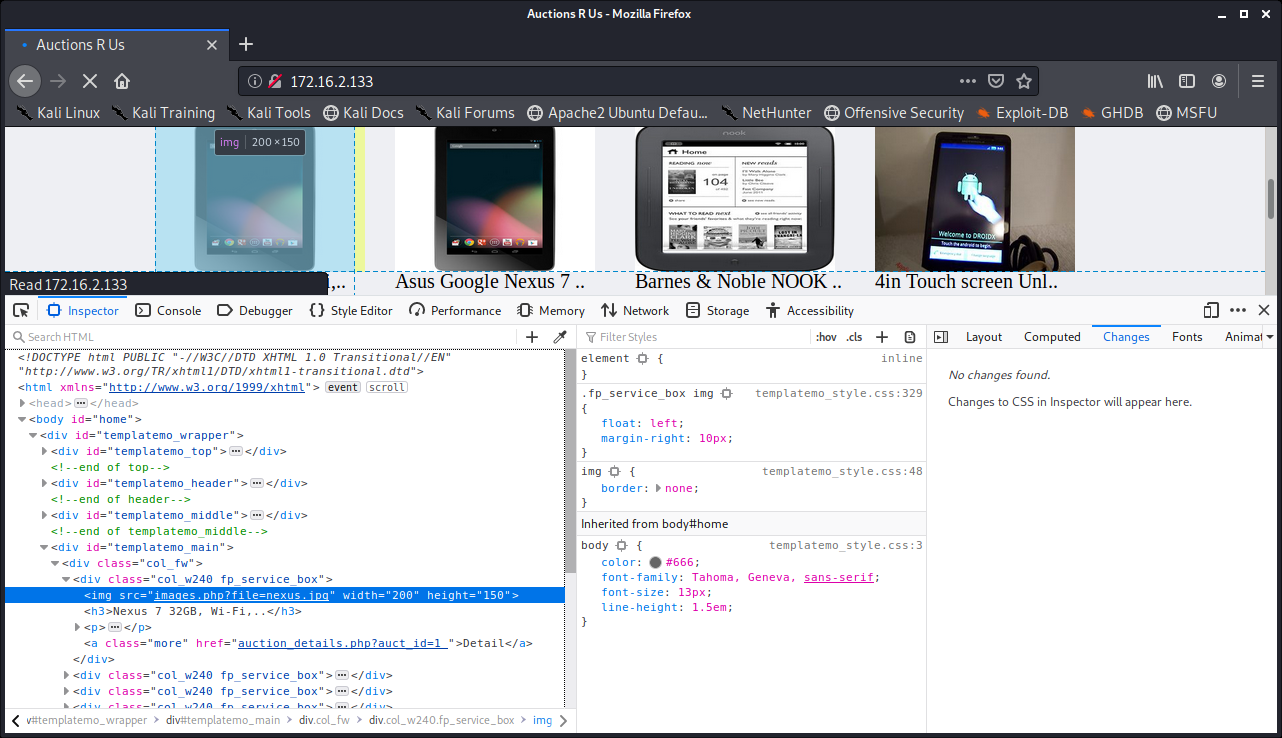
\includegraphics[scale=0.4]{img/pathtraversal1.png}
	\caption{Inspecting the image}
\end{figure}
\begin{figure}
	\centering
	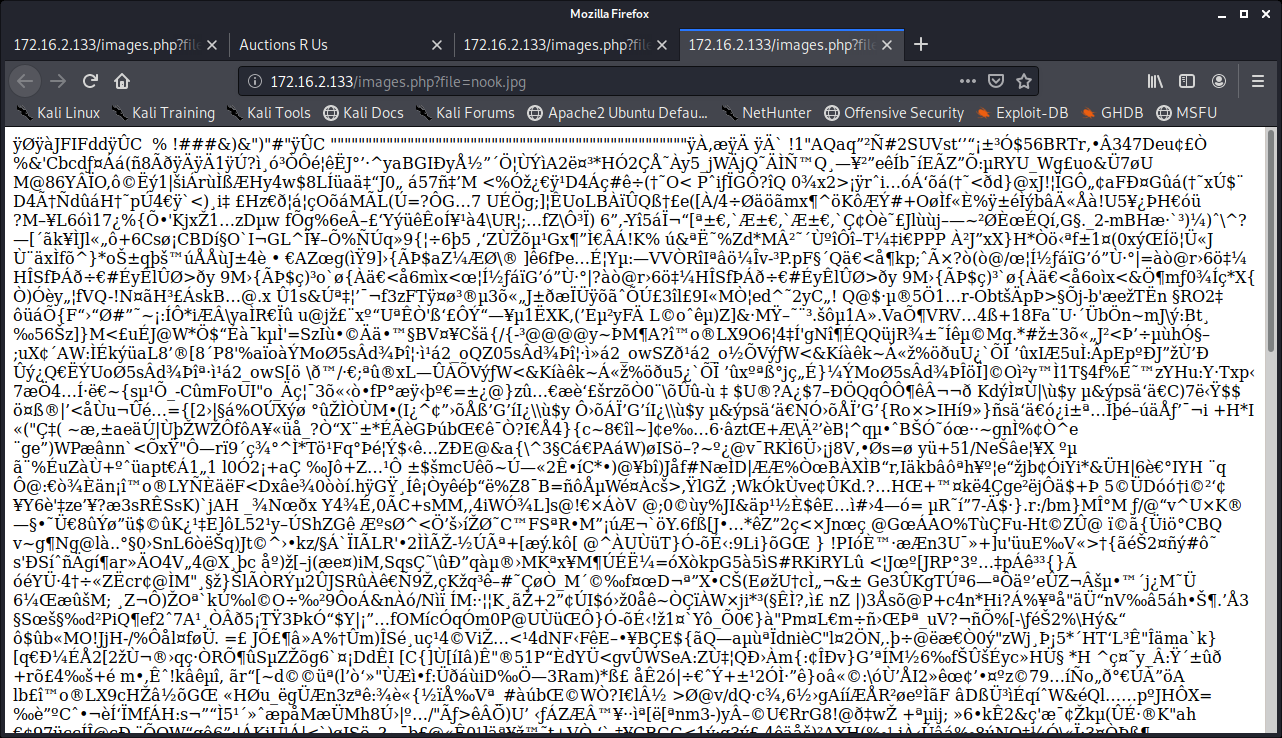
\includegraphics[scale=0.4]{img/pathtraversal2.png}
	\caption{Viewing the image contents}
\end{figure}
\begin{figure}
	\centering
	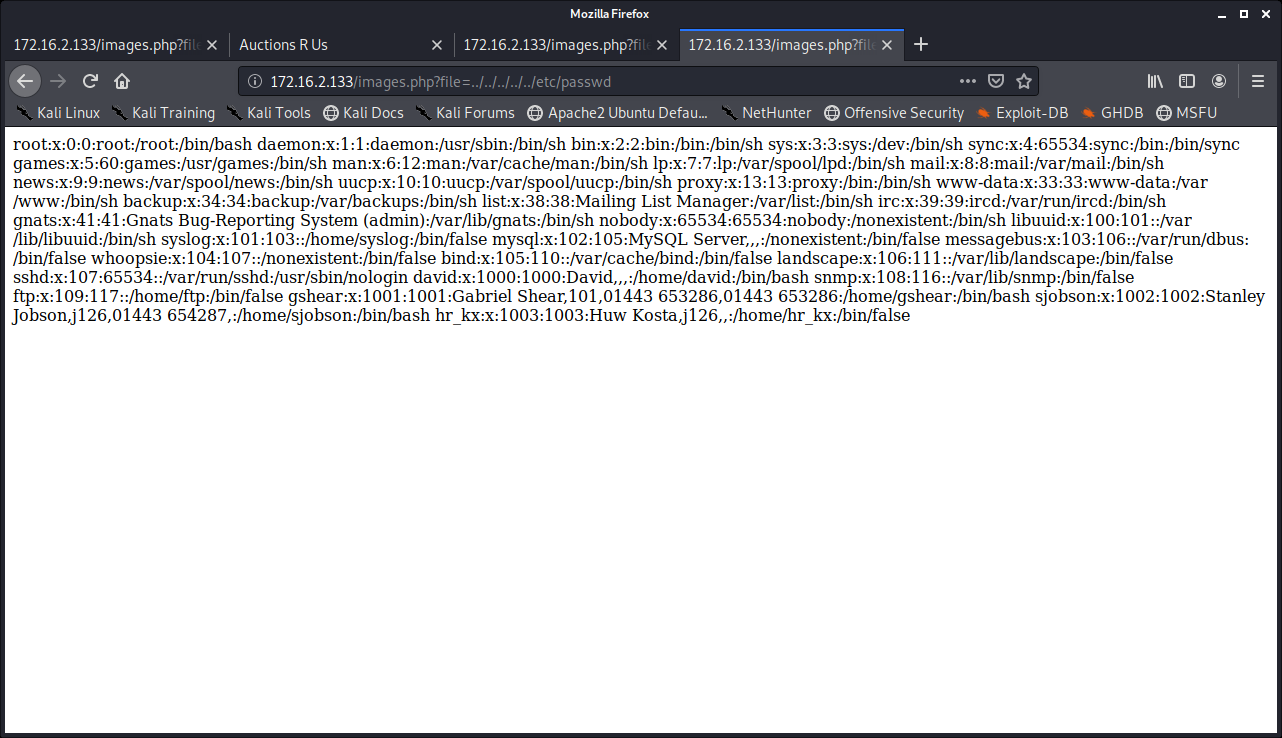
\includegraphics[scale=0.4]{img/pathtraversal3.png}
	\caption{Exploiting the file read}
\end{figure}
\subsection{SQL Injection}
\subsubsection{Security Implications / Risk Level}
\subsubsection{Cause of Vulnerability}
\subsubsection{Steps to Replicate}
\subsection{Weak Authentication}
\subsubsection{Security Implications / Risk Level}
\subsubsection{Cause of Vulnerability}
\subsubsection{Steps to Replicate}
\section{SRV1}
\section{SRV2}
\section{Ubuntu Client}

\chapter{Recommendations}
\section{Auction Site}
\section{SRV1}
\section{SRV2}
\section{Ubuntu Client}

\chapter{Conclusion}

\chapter{References}

\end{document}